\chapter{Introduction}
The \ac{IOT} is enabling communication among huge numbers of diverse low power devices.  
According to an estimate by Ericsson \cite{noauthor_internet_2017}, there will be 20 billion connected \ac{IOT} devices by 2023.
Modern communication protocols need to evolve rapidly to enable reliable connection among these devices.
The communication needs for a field temperature sensor differs from those of an industrial controller. 
Hence, there is need for research and development of communication protocols that satisfy these diverse device communication needs. 
The evaluation of these experimental protocols is difficult because of the need for specialized radio hardware.
Simulation is widely used to evaluate these protocols but they fall short on modeling of real world performance.
\ac{sdr} devices can be a powerful platforms for enabling the real-world evaluation of these protocols.\\

\ac{sdr} are flexible radio platforms where most of the communication systems functionality is designed in software. Typically, \ac{sdr} platforms have on board radio front-end equipped with wide band antennas and analog signal processing chain for tuning the carrier frequency and desired bandwidth. High speed data converters convert the incoming analog signals into the digital domain and vice versa. In traditional radios, the digital processing chain of a wireless protocol physical layer is implemented on the same chip as the radio front-end and analog signal processing functions. \ac{sdr}, on the other hand, in host-PHY \cite{nychis_enabling_nodate} architecture transfers the converted data to a general purpose computing platform using bus transfer (USB, PCIe). The digital processing chain is designed in software, thus allowing for flexibility in the protocol design, enabling experimentation in decoding and modulation techniques. \ac{sdr} also allows for careful analysis of RF signals as the raw sample data is made available to the host.
The key difference between \ac{sdr} and traditional radio has been shown in Figure \ref{sdr_architecture}. In both these radios data converters and analog frontend are designed on chip, with the traditional radios also including digital signal processing for a specific protocol on the same chip.
\\

\begin{figure}[!h]
\centering
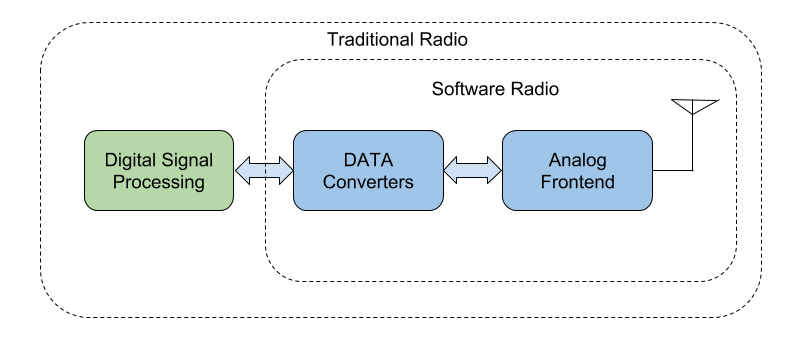
\includegraphics[width=0.75\textwidth]{Figure/SDRSystem.png}
\caption{Software Radio and Traditional Radio Architecture.}
\label{sdr_architecture}
\end{figure}


%\ac{sdr} helps to protect investments by facilitating change of protocols on already existing system. A major motivation within the commercial communications arena, is the rapid evolvement of communications standards, making software upgrades of base stations a more attractive solution than the costly replacement of base stations\cite{ulversoy_software_2010}. \ac{sdr} also opens up the possibility of Cognitive Radios, a context sensitive radio system that can adapt depending on the radio channel conditions and applications. \\

The movement of digital signal processing functions from hardware to software leads to performance issues in \ac{sdr} systems.
A fundamental challenge of an \ac{sdr} system is computational horsepower, because it needs to process complex data wave-forms in a reasonable time frame. Since \ac{sdr} involves transfer of signals and data from one system to another, considerable communication delays are introduced. Finally, general purpose processing systems introduces non-determinism in data processing, and communication processes.\\


\section{Problem Context}
Wireless devices share the wireless channel with other devices. The wireless protocol's \ac{mac} layer is responsible for moderating access to the wireless channel. It typically uses \ac{tdma} or \ac{csma} to allocate the use of the channel. \ac{tdma} protocols schedule the allocation of the entire channel to one of the devices for a particular time duration. This requires global time synchronization among the devices so that the devices can understand when to transmit and receive. \ac{csma}, on the other hand uses the channel on an opportunistic basis, with the devices sensing if the channel is free or not.\\

As highlighted by \cite{schmid_experimental_2007}, \ac{sdr} based systems don't comply with the stringent timing constraints imposed by modern \ac{mac} protocols. Furthermore, the presence of long bus communication and processing delays create blind spots \cite{schmid_experimental_2007} in carrier sensing. 
In Figure \ref{blind_spots}, the two problems originating from long delays are shown.
The left hand side image shows the problem of blind spots when using channel sensing for packet transmission.
The \ac{sdr} system wants to transmit a packet, so it uses channel sensing to detect when the channel is free.
An over the air packet ends at time $t_0$, this information is detected by the \ac{cpu} of the \ac{sdr} system after a certain delay, the channel sensing process keeps checking on the availability of the channel.
The channel information from time $t_1$ is used by the \ac{cpu} to infer that the channel is free and then starts the transmission.
The TX packet reaches the air medium at time $t_2$.
In case of \ac{sdr} systems this delay ($t_2-t_1$), can be quite significant.
This can result in collision with other nodes transmitting because of the communication and processing delays, the system is blind to real time channel situation.
In case of regular radio chips, the channel sensing logic is located very close to the \ac{RF} frontend, and the delay $t_2 - t_1$ is quite negligible, thereby resulting in smaller blind spots.\\

Another problem is illustrated in the right hand side image of Figure \ref{blind_spots}.
Because of larger communication and processing delays, it takes significantly longer for the \ac{sdr} system to acknowledge a received packet.
This acknowledgement time is referred to as \ac{IFS}.
The software implementation also introduces jitter in the {IFS}.
For a low powered radio node in \ac{IOT} applications, this jitter causes the radio to be turned on for significantly longer time.
The battery is drained away faster thereby undermining the purpose of minimal maintenance in \ac{IOT} systems.
Another problem with longer \ac{IFS} is lower spectral efficiency where the radio channel is unused for longer periods of time.\\ 

\begin{figure}[!h]
\centering
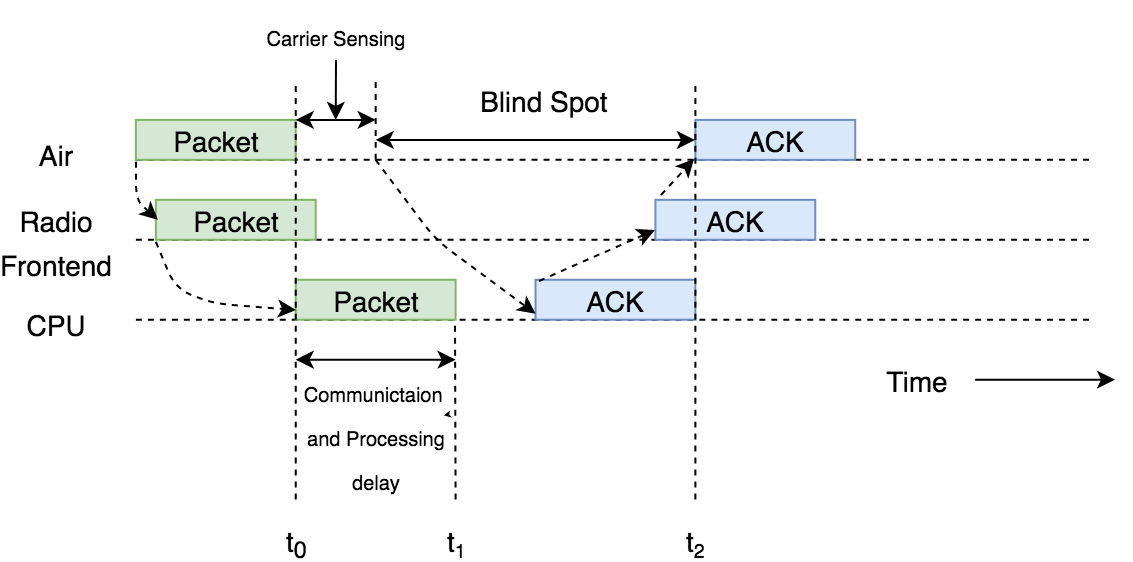
\includegraphics[width=\textwidth]{Figure/BlindSpots.png}
\caption{Problem Context Illustration (adapted from \cite{schmid_experimental_2007}).}
\label{blind_spots}
\end{figure}

The main problem with \ac{sdr} systems is long processing and buffering delays, which makes them non-compliant with most wireless protocols.
The characteristics of these delays needs to be understood to design \ac{mac} protocols which can take advantage of the flexibility provided by the \ac{sdr} platform taking into account the limitations of the platform.
% This necessitates a closer understanding of these delays and how different system parameters affect these delays.
%\subsection{TDMA}
%\ac{tdma} based protocols are controlled by time slots, hence there is need for precise scheduling to ensure that the transmissions happen in the correct time-slot. The delays and imprecise scheduling can be tolerated by making the time-slots longer but that degrades the efficiency of the overall network. Modern contention based protocols(\ac{csma}) also require precise timing to implement inter-frame spacing.\\

%Hence methods to implement precise time scheduling needs to studied.

\section{Project Context}

The project was conducted at RISE SICS as part of the 5G-Coral project \cite{noauthor_5g-coral_nodate}.
5G-Coral is an European Union H-2020 project which envisions a convergent radio access network.
The project visualizes numerous small multi-\ac{RAT} gateway handling traffic from different devices running different protocols to enable convergent access.
For the feasibility of this goal, the cost effectiveness of the radio-head needs to be taken into account.
LimeSDR \cite{noauthor_limesdr_nodate} provides a cost-effective \ac{sdr} platform, which supports the desired frequency bands making it the ideal choice as the project's radio-head.\\

Low power wireless devices are one of the main focus areas for the 5G-Coral project.
IEEE 802.15.4 is the most popular network specifications for \ac{LPWAN} i.e \ac{IOT} systems.
It specifically defines the physical Layer and the \ac{mac} layer of the network stack.
In order to successfully deploy flexible radio-head for \ac{LPWAN} devices, we need to understand the limitations and timing bottlenecks for this kind of system.
The lack of previous studies on the LimeSDR platform presents a knowledge gap which should be filled for future deployments using that platform.

%The lack of previous research on the characteristics of the platform made it the ideal choice for my \ac{sdr} platform.\\








\section{Research Question}
%\begin{itemize}
%\item{
Taking into consideration the problem and project context, we formulated this research question:
What are the characteristics of the delays introduced by different components in LimeSDR based IEEE 802.15.4 networks?\\
%}
\begin{figure}[!h]
\centering
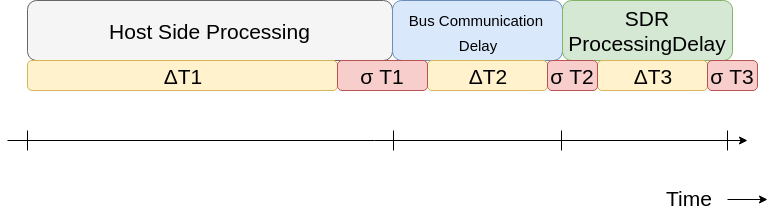
\includegraphics[width=0.75\textwidth]{Figure/RQ1.png}
\caption{Research Question}
\label{rq1}
\end{figure}

The research question is explained using Figure \ref{rq1} where the main components of the overall delay have been highlighted as host side processing, bus communication delay and SDR processing delay. 
Each of these components introduces a mean delay and jitter represented using yellow and red respectively in Figure \ref{rq1}.
The host side processing delay is introduced by running the software implementation of the 802.15.4 \ac{PHY} and \ac{mac} layers.
The bus communication delay represents the delay caused by the \ac{USB} 3.0 bus transfers.
The \ac{sdr} processing delay is the time required by the LimeSDR platform for transmission or reception of radio signals.
The objective of this thesis is to quantitatively evaluate these delays, $\Delta T_1$, $\Delta T_2$, $\Delta T_3$ etc as shown in Figure \ref{rq1}, and the impact of different network and \ac{sdr} configuration parameters on these delays.
%\item{ How to implement precise scheduling in LimeSDR based IEEE 802.15.4 communication system? }
%\end{itemize}

\section{Thesis Outline}
The thesis is structured as follows. \textit{Chapter 2} introduces the relevant background information for understanding the rest of the report.
Relevant previous work will be introduced in \textit{Chapter 3}.
\textit{Chapter 4} introduces the experimental setup and the methods used in the measurement of the timing delays.
The methods used in mitigation of these delays will be introduced in \textit{Chapter 5}.
\textit{Chapter 6} presents the results of the experiments and subjective analysis of these results.
Finally, \textit{Chapter 7} includes the concluding remarks and scope of future work.
